\documentclass[11pt,a4paper,oneside]{book}
\usepackage{fontspec}
\setmainfont{Noto Serif}
\setsansfont{Noto Sans}
\setmonofont{DejaVu Sans Mono}[Scale=.85]
\usepackage[english]{babel}
\usepackage{microtype}
\usepackage[a4paper,margin=21mm,top=22mm,bottom=24mm,headheight=15pt]{geometry}
\usepackage{amsmath,amssymb,mathtools,booktabs,tabularx,longtable,array,multirow}
\usepackage{enumitem,graphicx,tikz,hyperref,bookmark,multicol,needspace,fancyhdr,titlesec}
\usetikzlibrary{arrows.meta,positioning,shapes.geometric,calc,fit,backgrounds}
\usepackage[most]{tcolorbox}
\definecolor{Ink}{HTML}{202733}
\definecolor{Deep}{HTML}{14324A}
\definecolor{Blue}{HTML}{1C5D7A}
\definecolor{Teal}{HTML}{2E7D76}
\definecolor{Gold}{HTML}{B58135}
\definecolor{Brick}{HTML}{9C4F3E}
\definecolor{Paper}{HTML}{FBFAF7}
\definecolor{Mist}{HTML}{F1F4F4}
\definecolor{Warm}{HTML}{F7F1E7}
\definecolor{Muted}{HTML}{68717A}
\definecolor{PaleBlue}{HTML}{EAF1F4}
\definecolor{PaleTeal}{HTML}{EAF3F1}
\color{Ink}
\hypersetup{colorlinks=true,linkcolor=Deep,urlcolor=Blue,pdftitle={Kompyuter tarmoqlari va IP manzillash - attestatsiya nazariyasi}}
\setlength{\parindent}{1.1em}\setlength{\parskip}{3pt}\setlength{\emergencystretch}{2em}
\setlist[itemize]{leftmargin=1.3em,itemsep=2pt,topsep=3pt}
\setlist[enumerate]{leftmargin=1.5em,itemsep=2pt,topsep=3pt}
\newcolumntype{Y}{>{\raggedright\arraybackslash}X}
\renewcommand{\arraystretch}{1.2}
\renewcommand{\chaptermark}[1]{\markboth{\thechapter-bob. #1}{}}\pagestyle{fancy}\fancyhf{}\fancyhead[L]{\sffamily\small\color{Muted}\nouppercase{\leftmark}}\fancyhead[R]{\sffamily\small\color{Muted}\thepage}\renewcommand{\headrulewidth}{.3pt}
\fancypagestyle{plain}{\fancyhf{}\fancyfoot[C]{\sffamily\small\color{Muted}\thepage}\renewcommand{\headrulewidth}{0pt}}
\titleformat{\chapter}[display]{\sffamily\bfseries\color{Deep}}{\hfill\fontsize{58}{60}\selectfont\color{Deep!14}\thechapter}{-25pt}{\raggedright\fontsize{26}{31}\selectfont}[\vspace{5pt}\color{Gold}\titlerule]
\titleformat{\section}{\Large\sffamily\bfseries\color{Deep}}{\thesection}{.7em}{}
\titleformat{\subsection}{\normalsize\sffamily\bfseries\color{Blue}}{\thesubsection}{.7em}{}
\newtcolorbox{goal}{enhanced,breakable,colback=PaleBlue,colframe=PaleBlue,boxrule=0pt,borderline west={2pt}{0pt}{Blue},arc=0mm,title={\sffamily\bfseries Bob maqsadi},coltitle=Deep}
\newtcolorbox{tip}[1]{enhanced,breakable,colback=PaleTeal,colframe=PaleTeal,boxrule=0pt,borderline west={2pt}{0pt}{Teal},arc=0mm,title={\sffamily\bfseries #1},coltitle=Teal}
\newtcolorbox{caution}[1]{enhanced,breakable,colback=Warm,colframe=Warm,boxrule=0pt,borderline west={2pt}{0pt}{Gold},arc=0mm,title={\sffamily\bfseries #1},coltitle=Deep}
\newtcolorbox{worked}[1]{enhanced,breakable,colback=white,colframe=Deep!35,boxrule=.5pt,arc=0mm,title={\sffamily\bfseries #1},coltitle=Deep}
\newcommand{\src}[1]{\par\smallskip{\footnotesize\sffamily\color{Muted}Manba izi: #1}\par}
\newcommand{\kw}[1]{\textbf{\color{Deep}#1}}
\newcommand{\ip}[1]{\texttt{#1}}
\newcommand{\summarybox}[1]{\begin{tip}{Bob xulosasi}#1\end{tip}}
\begin{document}
\begin{titlepage}
\begin{tikzpicture}[remember picture,overlay]
\fill[Deep](current page.south west) rectangle (current page.north east);
\fill[Blue]([xshift=13mm]current page.south west) rectangle ([xshift=30mm]current page.north west);
\fill[Gold]([xshift=30mm]current page.south west) rectangle ([xshift=33mm]current page.north west);
\node[anchor=north east,text=white!9,font=\sffamily\bfseries\fontsize{136}{136}\selectfont]at ([xshift=3mm,yshift=-10mm]current page.north east){06};
\end{tikzpicture}
\vspace*{23mm}\hspace*{25mm}{\sffamily\color{white!77}\large INFORMATIKA ATTESTATSIYASI \textbullet\ 2026\par}
\vspace{37mm}
\hspace*{25mm}\begin{minipage}{140mm}
{\sffamily\bfseries\color{white}\fontsize{29}{34}\selectfont KOMPYUTER\par TARMOQLARI VA\par TARMOQ ARXITEKTURASI\par}
\vspace{8mm}{\sffamily\color{white!88}\fontsize{19}{25}\selectfont IP MANZILLASH VA INTERNETDA ISHLASH\par}
\vspace{14mm}{\color{white!76}\large Qayta ishlangan nazariy qo'llanma: tushuncha \(\to\) farqlash \(\to\) hisoblash \(\to\) attestatsiya vaziyati\par}
\end{minipage}
\vfill\hspace*{25mm}{\sffamily\color{white!75}10 bob \textbullet\ kengaytirilgan manba izlari \textbullet\ IP yechimlari\par}
\hspace*{25mm}{\sffamily\color{white!60}Toshkent, 2026\par}
\end{titlepage}
\frontmatter
\chapter*{Nashr pasporti}\addcontentsline{toc}{chapter}{Nashr pasporti}
\par\medskip
\par\medskip
\begin{tabularx}{\textwidth}{p{.27\textwidth}Y}\toprule
Maqsad & Informatika attestatsiyasi, 2026-yil spetsifikatsiyasi, 6-mazmun sohasi, 32--33-savollarga tayyorgarlik.\\
Asosiy darslik & 11-sinf Informatika va axborot texnologiyalari (2021), 19--31-darslar, kitobdagi 129--196-betlar.\\
Qo'shimcha darsliklar & 6-sinf (2021), 17--20-darslar; 5--11-sinf Cambridge moslashtirilgan nashrlari; 11-sinf axborot xavfsizligi darslari.\\
Mazmunning maqomi & Darsliklardan sintez qilingan ta'riflar va vaziyatlar; CIDR, broadcast, maxsus IP diapazonlari va protokollar bo'yicha aniqlashtirishlar alohida belgilangan.\\
Test formati & Yagona javobli testlar (Y1), moslashtirish (Y2), ketma-ketlik (Y3), izohli o'qituvchi va javobsiz o'quvchi nusxasi.\\
\bottomrule\end{tabularx}
\begin{caution}{Muhim ilmiy izoh}
11-sinf darsligida \ip{127.0.0.0/8} diapazoni xususiy manzillar yaqinida sanaladi. Zamonaviy IPv4 amaliyotida bu \emph{loopback}, ya'ni mahalliy qaytish manzillari oralig'idir; RFC~1918 xususiy manzil diapazoniga kirmaydi. Internetda marshrutlanmaydigan har bir manzilni ham RFC~1918 xususiy manzil deb atash xato. Ushbu qo'llanma tarixiy sinfli IP va zamonaviy CIDR tushunchalarini ham ajratadi.
\end{caution}
\tableofcontents
\mainmatter
\chapter{Kompyuter tarmog'i va uning turlari}
\begin{goal}Tarmoqni, uning tarkibiy qismlarini va hududiy turlarini aniqlash; tarmoq tanlash vaziyatlarini izohlash.\end{goal}
\section{Ta'rif, vazifa va resurslar}
\kw{Kompyuter tarmog'i} — kompyuterlar va boshqa raqamli qurilmalarni aloqa kanallari hamda tegishli apparat-dasturiy vositalar orqali bog'lab, ma'lumot almashish va resurslardan birgalikda foydalanishni ta'minlovchi tizim. \kw{Tugun} (node) — tarmoqqa ulangan element; \kw{xost} (host) odatda manzillanadigan yakuniy qurilma; \kw{server} — boshqa ishtirokchilarga xizmat ko'rsatuvchi tizim. Bitta jismoniy server bir necha xizmatni, bitta xizmat esa bir necha serverda bajarilishi mumkin.

Tarmoqqa ulanishning maqsadlari: fayl almashish, markazlashgan saqlash, umumiy printer, internetga chiqish, elektron muloqot, zaxiralash, masofaviy ishlash. Cheklovlari: dastlabki xarajat, boshqaruv va xavfsizlik talablari, markaziy nuqtaga qaramlik, tarmoqdagi nosozlik ta'siri.
\begin{tip}{Atamalarni ajrating}Internet — dunyo miqyosidagi o'zaro bog'langan IP tarmoqlari; lokal tarmoq esa internetga ulanmasdan ham ishlashi mumkin. Wi-Fi — simsiz lokal tarmoqqa ulanish texnologiyasi, internetning sinonimi emas.\end{tip}
\section{Tarmoqning tarkibi}
\par\medskip
\par\medskip
\begin{tabularx}{\textwidth}{p{.24\textwidth}Y}\toprule
Tarkib & Vazifa\\\midrule
Yakuniy qurilma & Noutbuk, telefon, printer, server; ma'lumot yaratadi, oladi yoki xizmat ko'rsatadi.\\
Tarmoq interfeysi (NIC) & Qurilmani Ethernet yoki Wi-Fi tarmog'iga ulaydi; odatda kanal darajasida MAC manzili mavjud.\\
Uzatish muhiti & Mis kabel, optik tola yoki radioto'lqin; signal shu muhit orqali tarqaladi.\\
Oraliq qurilma & Switch, router, access point, modem va boshqalar; uzatish hamda yo'naltirishga yordam beradi.\\
Tarmoq dasturi/protokol & Qurilmalar o'zaro qanday muloqot qilishini belgilaydi.\\\bottomrule\end{tabularx}
\section{Hududiy turlar}
\par\medskip
\par\medskip
\begin{tabularx}{\textwidth}{p{.19\textwidth}Y p{.27\textwidth}}\toprule
Tur & Qamrov va mazmun & Misol\\\midrule
PAN/WPAN & Shaxsning yaqin atrofidagi qurilmalar; ko'pincha Bluetooth. & Telefon va quloqchin.\\
HAN & Uy ichidagi tarmoq. & Uy routeriga ulangan qurilmalar.\\
LAN/WLAN & Xona, bino, kampusning mahalliy segmenti; WLAN simsiz LAN. & Maktab kompyuter xonasi.\\
MAN & Shahar miqyosidagi bog'lanish. & Shahardagi bir necha filial.\\
WAN & Katta geografik masofadagi tarmoqlarni bog'lash. & Turli viloyatlardagi filiallar.\\
Internet & Mustaqil IP tarmoqlarining global birlashmasi. & Umumjahon internet.\\\bottomrule\end{tabularx}
\begin{caution}{Shartga qarab javob}
Tarmoq turi faqat kabelning mavjudligi bilan belgilanmaydi. \emph{WLAN} ham lokal tarmoq; \emph{WAN} doimo simsiz degani emas. Bir tashkilotning bir shahardagi turli manzillari LAN, MAN yoki WAN arxitekturasi yordamida bog'lanishi mumkin: testdagi aniq qamrov va aloqa usulini tekshiring.
\end{caution}

\section{Internet, intranet va extranet chegaralari}
\kw{Internet} --- turli tashkilotlarga qarashli IP tarmoqlarining global birlashmasi. \kw{Intranet} --- tashkilot ichidagi xodimlar uchun mo'ljallangan, ko'pincha veb-texnologiyalardan foydalanuvchi cheklangan resurslar muhiti. \kw{Extranet} --- tashkilotning ayrim ichki resurslariga ruxsat etilgan tashqi hamkorlarni nazorat bilan kiritish shakli. \emph{Intranet} faqat Internetdan uzilgan alohida kabel bo'lishi shart emas: tashkilot VPN kabi himoyalangan kanal orqali masofadagi xodimga intranet kirishini berishi mumkin.
\par\medskip
\begin{tabularx}{\textwidth}{p{.22\textwidth}Y Y}\toprule
Tushuncha & Asosiy auditoriya & Vaziyat\\\midrule
Internet & Umumiy ochiq global infratuzilma & Ommaviy veb-sayt\\
Intranet & Ichki ruxsatli xodimlar & Maktabning ichki hujjat portali\\
Extranet & Ruxsatli tashqi hamkor & Ta'minotchiga cheklangan buyurtma portali\\\bottomrule\end{tabularx}
\begin{worked}{Bir bino, uch xizmat}
O'quvchi ommaviy ta'lim portalini ochadi (Internet), o'qituvchi maxsus login bilan maktabning ichki jadvaliga kiradi (intranet), tashqi ta'minotchi buyurtmaning faqat o'ziga tegishli qismini ko'radi (extranet). Uchchala xizmat ham IP/veb protokollaridan foydalanishi mumkin; farq --- ruxsat va auditoriya.
\end{worked}
\src{M11, darslikning 136--138-betlari, 19--20-darslar (intranet); extranet --- mavzuga oid qo'shimcha aniqlashtirish.}
\section{Simli va simsiz tarmoq}
Simli Ethernetda odatiy muhit — o'ralgan juftlik (UTP/STP) yoki optik tola. Simsiz WLAN radiokanaldan foydalanadi. Simli ulanish barqarorlik va boshqariladigan fizik kirishni ta'minlashi mumkin; Wi-Fi qurilma harakatchanligiga qulay. Haqiqiy unumdorlik signal, masofa, xalaqit, foydalanuvchilar soni va uskunaga bog'liq.
\begin{worked}{Vaziyat}
Maktab binosidagi 20 ta kompyuter bitta printerni ulashib ishlatadi. Internet uzilib qoldi, lekin lokal switch va printer ishlayapti. Lokal printer ishlashda davom etishi mumkin: \emph{LAN} va \emph{internet} bir xil emas.
\end{worked}
\src{M11, 129--139-betlar (19--20-darslar); C11, tarmoqlar bo'limi.}
\summarybox{PAN — shaxsiy; LAN — mahalliy; MAN — shahar; WAN — uzoq masofa. Tarmoqdan foydalanish internetga chiqish bilangina cheklanmaydi.}

\chapter{Tarmoq qurilmalari va uzatish muhiti}
\begin{goal}Har bir qurilmani unga mos vazifa va darajada farqlash; tarmoq vaziyatida to'g'ri qurilmani tanlash.\end{goal}
\section{Asosiy qurilmalar}
\par\medskip
\begin{longtable}{p{.19\textwidth}p{.46\textwidth}p{.26\textwidth}}\toprule
Qurilma & Asosiy vazifa & Nozik farq\\\midrule\endhead
\kw{NIC} & Kompyuterga tarmoq interfeysi taqdim etadi. & IP va MAC aynan bir narsa emas.\\
\kw{Hub} & Kelgan bit/signalni boshqa portlarga qayta uzatadi. & Manzil bo'yicha tanlab yubormaydi.\\
\kw{Switch} & Ethernet freymlarini MAC jadvallari yordamida kerakli portga uzatadi. & Oddiy Layer 2 switch — marshrutizator emas.\\
\kw{Router} & IP paketlarni turli IP tarmoqlari orasida yo'naltiradi. & Default gateway ko'pincha router interfeysi.\\
\kw{Access point} & Simsiz klientlarni LANga ulaydi. & AP har doim router bo'lishi shart emas.\\
\kw{Modem} & Provayderning kirish kanaliga xos signal/interfeysni moslashtiradi. & Modem, router va Wi-Fi AP turli vazifa.\\
\kw{Repeater} & Signalni regeneratsiya/uzoqroq uzatishga yordam beradi. & Paketlarni IP bo'yicha marshrutlamaydi.\\
\kw{Bridge} & Ikki kanal segmentini MAC darajasida bog'laydi. & Zamonaviy switch ko'p portli ko'prikka yaqin.\\
\kw{Firewall} & Belgilangan qoidalar bo'yicha trafikni nazorat/filtr qiladi. & Alohida qurilma yoki dastur bo'lishi mumkin.\\
\kw{Server} & Fayl, veb, DNS, DHCP kabi xizmatlarni beradi. & Qurilma roli mantiqiy; server oddiy kompyuter ham bo'lishi mumkin.\\\bottomrule
\end{longtable}

\section{Server turlari va tarmoqdagi dasturiy komponentlar}
11-sinf darsligida tarmoqning \kw{texnik komponentlari} sifatida abonent qurilmalari, aloqa kanallari, adapter, kommutator, ko'prik va router; \kw{dasturiy komponentlari} sifatida tarmoq operatsion tizimlari va ulanishni ta'minlovchi protokol-xizmatlar ajratilgan. Misollar: Windows Server/Linux kabi tizimlar, tarmoq mijozi, fayllarni ulashish va masofaviy kirish xizmatlari. Tarmoq operatsion tizimi apparat qurilma emas.
\par\medskip
\begin{tabularx}{\textwidth}{p{.25\textwidth}Y}\toprule
Server turi & Qanday xizmat ko'rsatadi?\\\midrule
Fayl-server & Umumiy fayllarni saqlash va ruxsat bilan ulashish\\
Print-server & Chop etish so'rovlarini navbatlash va printerdan umumiy foydalanish\\
Veb-server & HTTP(S) so'rovlariga veb-resurs yuborish\\
Pochta serveri & Xatni uzatish, qabul qilish yoki qutini saqlash\\
Ma'lumotlar bazasi serveri & So'rov asosida markazlashgan ma'lumotga kirish\\\bottomrule\end{tabularx}
\begin{caution}{Server tushunchasini yoddan chiqarmang}
\emph{Server} ko'p hollarda xizmatni bajaruvchi dastur yoki shu dasturni ishlatayotgan kompyuter degani. ``Har bir xizmat uchun alohida jismoniy kompyuter shart'' va ``har bir server internetdagi ommaga ochiq'' kabi hukmlar noto'g'ri. Mijoz-server modeli topologiya bilan aynan bir xil emas.
\end{caution}
\src{M11, 140--145-betlar (21-dars), 160--163-betlar (tarmoq dasturiy ta'minoti); C8, kompyuter tarmog'i moduli, PDF 91--113-betlar.}
\section{Kadr (frame) va paket (packet)}
Ethernet kommutatori odatda freymdagi \kw{MAC} manziliga, router esa paketdagi \kw{IP} manziliga qarab qaror qabul qiladi. IP manzili tarmoqqa qarab o'zgarishi mumkin; MAC interfeysning kanal darajasidagi identifikatoridir. Ushbu farq testda ko'p chalg'itadi.
\begin{center}
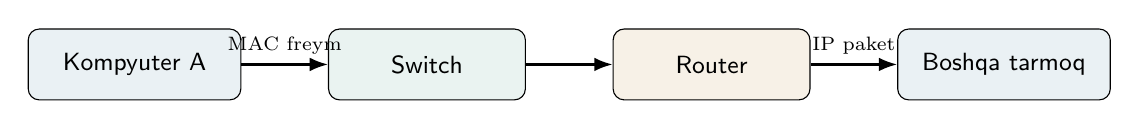
\begin{tikzpicture}[every node/.style={font=\small\sffamily},node distance=11mm]
\node[draw,rounded corners,fill=PaleBlue,minimum width=27mm,minimum height=9mm](a){Kompyuter A};
\node[draw,rounded corners,fill=PaleTeal,right=of a,minimum width=25mm,minimum height=9mm](s){Switch};
\node[draw,rounded corners,fill=Warm,right=of s,minimum width=25mm,minimum height=9mm](r){Router};
\node[draw,rounded corners,fill=PaleBlue,right=of r,minimum width=27mm,minimum height=9mm](b){Boshqa tarmoq};
\draw[-{Latex},thick](a)--node[above,font=\scriptsize]{MAC freym}(s);
\draw[-{Latex},thick](s)--(r);
\draw[-{Latex},thick](r)--node[above,font=\scriptsize]{IP paket}(b);
\end{tikzpicture}
\end{center}
\section{Aloqa vositalari}
\par\medskip
\par\medskip
\begin{tabularx}{\textwidth}{p{.24\textwidth}Y}\toprule
Muhit & Amaliy xususiyat\\\midrule
O'ralgan juft kabel & Ethernet LAN; RJ-45 ulagich ko'p uchraydi. UTP va STP ekranlanganlik bilan farqlanadi.\\
Optik tolali kabel & Ma'lumotni yorug'lik impulslarida uzatadi; elektromagnit shovqinga chidamli, uzoq masofa uchun qulay.\\
Koaksial kabel & Tarixiy LAN va ayrim provayder aloqa kanallarida qo'llanadi.\\
Radio (Wi-Fi/Bluetooth) & Simsiz va qulay; radiochastota, to'siq va xalaqitga sezgir.\\\bottomrule\end{tabularx}
\begin{worked}{Uch xil nosozlik}
1) Bir lokal xonada yangi kompyuter uchun bo'sh Ethernet port kerak: \textbf{switch}. 2) \ip{192.168.1.0/24} dan \ip{192.168.2.0/24} ga trafik: \textbf{router}. 3) Simsiz telefonlarni mavjud simli LANga ulash: \textbf{access point}.
\end{worked}
\begin{caution}{Bir qutida bir necha vazifa}
Uy uchun sotiladigan ``Wi-Fi router'' odatda router + switch + access point + ba'zan modem funksiyalarini o'z ichiga oladi. Qurilmaning savdo nomidan emas, savolda talab qilingan \emph{funksiyadan} kelib chiqing.
\end{caution}
\src{M11, 156--166-betlar (24--25-darslar); C11, 13-bob, tarmoq komponentlari.}
\summarybox{Switch — MAC bo'yicha LAN ichida; router — IP bo'yicha tarmoqlar orasida; AP — simsiz kirish; modem — kanalga moslash.}


\section{Aloqa kanallarining kengaytirilgan tasnifi}
\kw{Simli muhitlar}: o'ralgan juftlik UTP/STP (mis), koaksial kabel (mis), optik tola (yorug'lik). \kw{Simsiz muhitlar}: qisqa masofali Bluetooth, Wi-Fi (WLAN), uyali mobil aloqa, radiorele/mikroto'lqin, infraqizil aloqa va sun'iy yo'ldosh kanali. Tarmoq turi (LAN/WAN) bilan signal muhiti (simli/simsiz) --- ikki mustaqil mezon.
\par\medskip
\begin{tabularx}{\textwidth}{p{.22\textwidth}p{.37\textwidth}Y}\toprule
Muhit & Afzallik & Cheklov yoki vaziyat\\\midrule
UTP/STP & Keng tarqalgan LAN ulanishi & Misda xalaqit va masofa hisobga olinadi; STP ekranli\\
Optik tola & Elektromagnit xalaqitga chidamli; katta hajm & Optik transiver va montaj talab qiladi\\
Koaksial & Ekranli mis kabel & Kabel TV va ayrim eski tarmoqlarda\\
Wi-Fi & Qulay mobil ulanish & Radio shovqin, devorlar, xavfsizlik sozlamalari\\
Uyali aloqa & Operator qamrovida mobillik & Qamrov va tarifga bog'liq\\
Sun'iy yo'ldosh & O'zaro juda uzoq/yetib borish qiyin hududlar & Kechikish va atmosfera ta'siri turlicha\\\bottomrule\end{tabularx}
\begin{worked}{Kanal tanlash}
Maktab binolari orasida elektromagnit shovqin kuchli va kabel masofasi uzun. Optik tola mos bo'lishi mumkin. Harakatdagi planshetlar uchun AP orqali Wi-Fi qulay. Uzoq qishloq hududida yer usti magistrali yo'q bo'lsa, sun'iy yo'ldosh yoki mobil operator aloqa varianti baholanadi; har birini narx, qamrov, uzilish xavfi va tezlik bilan solishtiring.
\end{worked}
\src{M11, 146--155-betlar (22--23-dars), simli/simsiz aloqa texnologiyalari; C8, PDF 91--113-betlar.}

\chapter{Tarmoq arxitekturasi va topologiyasi}
\begin{goal}Mijoz-server va P2P modelini hamda fizik/mantiqiy topologiyani farqlash; nosozlik nuqtalarini tahlil qilish.\end{goal}
\section{Mijoz-server va teng huquqli model}
\kw{Client--server}: mijoz (client) so'rov yuboradi, server javob beradi yoki resursni taqdim etadi. Markaziy autentifikatsiya, yagona zaxira va boshqaruv uchun qulay; server yoki ulanishdagi nosozlik xizmatni cheklashi mumkin. \kw{Peer-to-peer (P2P)}: qurilmalar bir-biriga teng darajada bevosita xizmat ko'rsatishi mumkin. Kichik tarmoqlarda sodda; markazlashgan ruxsat va boshqaruv murakkabroq bo'lishi mumkin.
\par\medskip
\par\medskip
\begin{tabularx}{\textwidth}{p{.23\textwidth}YY}\toprule
Mezon & Client--server & P2P\\\midrule
Resurs & Ko'pincha markazlashgan & Ishtirokchilar o'rtasida\\
Boshqaruv & Yagona siyosatni joriy etish qulay & Har bir tugunda alohida bo'lishi mumkin\\
Misol & Maktab domenida fayl serveri & Ikki kompyuterning fayl almashishi\\\bottomrule\end{tabularx}
\section{Topologiya: ulanish sxemasi}
\kw{Fizik topologiya} — qurilmalar va aloqa kanallarining jismoniy joylashuvi; \kw{mantiqiy topologiya} — ma'lumot oqimi va aloqa tartibi. Turli mantiqiy ishlashlar bir xil fizik chizmada amalga oshishi mumkin.
\par\medskip
\par\medskip
\begin{tabularx}{\textwidth}{p{.19\textwidth}YY}\toprule
Topologiya & Asosiy belgisi & Nosozlikdagi xatar\\\midrule
Shina (bus) & Umumiy magistral kabel & Magistral uzilsa ko'p tugun ta'sirlanadi.\\
Halqa (ring) & Tugunlar yopiq zanjir & Oddiy halqada bir uzilish muammoli; zaxira halqa bo'lishi mumkin.\\
Yulduz (star) & Har tugun markaziy switchga ulanadi & Markaziy qurilma yagona xato nuqtasi.\\
To'rli (mesh) & Tugunlar orasida bir nechta yo'l & Yuqori chidamlilik, ammo ko'p aloqa talab etishi mumkin.\\
Daraxt (tree) & Ierarxik yulduzlar & Yuqori bosqich qurilmasi quyi qismlarga ta'sir qilishi mumkin.\\
Gibrid & Bir necha topologiya aralashmasi & Xatar tanlangan segmentlar strukturasiga bog'liq.\\\bottomrule\end{tabularx}
\begin{center}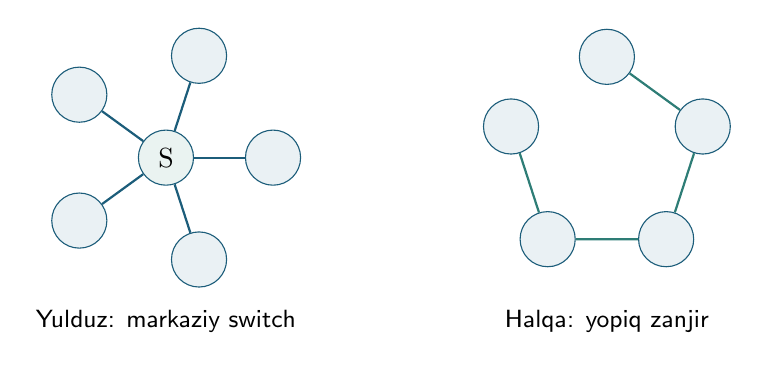
\begin{tikzpicture}[scale=.8,every node/.style={circle,draw=Blue,fill=PaleBlue,inner sep=3pt,minimum size=7mm}]
\node[fill=PaleTeal](c)at(0,0){S};
\foreach \a in {0,72,144,216,288}{\node(n\a)at(\a:1.7){};\draw[thick,Blue](c)--(n\a);}
\node[draw=none,fill=none,rectangle]at(0,-2.6){\small\sffamily Yulduz: markaziy switch};
\begin{scope}[xshift=7cm]
\foreach \a in {90,18,-54,-126,-198}{\node(m\a)at(\a:1.6){};}
\draw[thick,Teal](m90)--(m18)--(m-54)--(m-126)--(m-198)--cycle;
\node[draw=none,fill=none,rectangle]at(0,-2.6){\small\sffamily Halqa: yopiq zanjir};
\end{scope}
\end{tikzpicture}\end{center}

\section{Sxemani o'qish: fizik va xizmat arxitekturasi}
\begin{center}
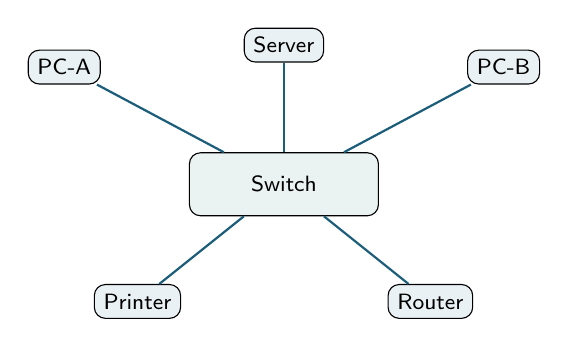
\begin{tikzpicture}[scale=.93, every node/.style={font=\footnotesize\sffamily}]
\node[draw,rounded corners,fill=PaleTeal,minimum width=24mm,minimum height=8mm] (sw) at (0,0) {Switch};
\node[draw,rounded corners,fill=PaleBlue] (a) at (-3,1.6) {PC-A};
\node[draw,rounded corners,fill=PaleBlue] (b) at (0,1.9) {Server};
\node[draw,rounded corners,fill=PaleBlue] (c) at (3,1.6) {PC-B};
\node[draw,rounded corners,fill=PaleBlue] (d) at (-2,-1.6) {Printer};
\node[draw,rounded corners,fill=PaleBlue] (e) at (2,-1.6) {Router};
\foreach \x in {a,b,c,d,e}{\draw[thick,Blue] (sw)--(\x);}
\end{tikzpicture}
\end{center}
Rasmda barcha chekka tugunlar markaziy switchga ulanadi: \kw{fizik topologiya --- yulduz}. Server markazda chizilmagani sababli uning xizmat roli kamaymaydi: \kw{mijoz/server} arxitekturasi alohida masala. Router boshqa IP tarmoqqa o'tish uchun kerak bo'lishi mumkin, lekin faqat bitta LAN printerini ulashish uchun doimo shart emas.
\src{M11, 140--145, 167--171-betlar; sxema --- sintez qilingan mashq.}
\section{To'liq mesh uchun bog'lanishlar soni}
Agar $n$ ta tugunning \emph{har bir jufti} alohida ikki tomonlama aloqa bilan bog'lansa, qirralar soni
\[E=\frac{n(n-1)}{2}.\]
\begin{worked}{Hisoblash}
6 ta tugunli to'liq meshda $E=6\cdot5/2=15$ ta aloqa bor. Bu formula shina, yulduz yoki qisman mesh uchun bevosita qo'llanmaydi.
\end{worked}
\begin{caution}{Halqa haqida mutlaq hukm qilmang}
Oddiy yagona halqada bir uzilish aloqa to'xtashiga olib kelishi mumkin; lekin zaxiralangan halqa protokollarida boshqa yo'l bor. Test ``oddiy halqa'' deyaptimi yoki ortiqcha yo'l mavjudligini ko'rsatyaptimi — aniqlang.
\end{caution}
\src{M11, 140--145 va 167--171-betlar (21 va 26-darslar); C11, tarmoq arxitekturasi.}
\summarybox{Mijoz-server — rollar; yulduz/halqa/shina — ulanish shakli. Bu ikki tasnifni bir-biriga almashtirmang.}

\chapter{Tarmoqlarning ishlash prinsipi va protokollar}
\begin{goal}Uzatish yo'lini, qatlamlarni va TCP/IP oilasining vazifalarini ajratish; muammolarni qatlamga bog'lash.\end{goal}
\section{Paketli uzatish}
Ma'lumot kichik birliklarga ajratilib, sarlavhalar bilan uzatilishi mumkin. \kw{IP paketi} tarmoqlar o'rtasida yetkaziladi; \kw{Ethernet freymi} lokal kanal bo'ylab uzatiladi; \kw{TCP segmenti} transport darajasidagi ma'lumotni tashiydi. Turli qatlamlarda ``paket'' so'zi umumiy ma'noda ishlatilsa ham, attestatsiyada qaysi sarlavha qaysi darajaga tegishli ekanini ajrating.
\section{Soddalashtirilgan TCP/IP modeli}
\par\medskip
\par\medskip
\begin{tabularx}{\textwidth}{p{.22\textwidth}p{.31\textwidth}Y}\toprule
Qatlam & Vazifa & Misollar\\\midrule
Ilova & Foydalanuvchi xizmatlari va so'rovlar & HTTP(S), DNS, SMTP, IMAP, DHCP\\
Transport & Dasturlar o'rtasida uzatish & TCP, UDP, portlar\\
Internet & Tarmoqlararo manzillash va yo'naltirish & IPv4, IPv6, ICMP\\
Kanal va fizik & Mahalliy kadr va signal uzatish & Ethernet, Wi-Fi, MAC, optik kabel\\\bottomrule\end{tabularx}
\section{TCP va UDP farqi}
\kw{TCP} ulanishni o'rnatadi, tartib va yo'qolgan ma'lumotlarni qayta uzatishni boshqaradi; \kw{UDP} bog'lanishsiz datagrammalarni yuboradi va TCPdagi kafolatlarni o'zida bermaydi. UDP ishlatilgan xizmat ham ilova darajasida nazorat mexanizmlariga ega bo'lishi mumkin. ``UDP har doim tez'' yoki ``TCP har doim sekin'' — mutlaq to'g'ri emas.
\section{IP, MAC, port va DNS}
\par\medskip
\par\medskip
\begin{tabularx}{\textwidth}{p{.20\textwidth}Y}\toprule
Atama & Asosiy savolga javob\\\midrule
MAC & Shu lokal kanal ichida qaysi interfeys?\\
IP & Qaysi tarmoqdagi qaysi interfeys?\\
Port & Qaysi xizmat/dastur muloqotining oxirgi nuqtasi?\\
DNS & Domen nomiga mos manzilni qanday topamiz?\\\bottomrule\end{tabularx}
\section{Tarmoqdan tashqariga uzatish yo'li}
\begin{enumerate}
\item Kompyuter maska asosida qabul qiluvchining manzili o'z subnetidami-yo'qmi tekshiradi.
\item Bir subnetda bo'lsa, lokal aloqa uchun kerakli MAC aniqlanadi (IPv4da ARP).
\item Boshqa subnetda bo'lsa, paket \kw{default gateway}ga yuboriladi; IP manzil qabul qiluvchining o'ziniki bo'lib qoladi, lokal Ethernet freymi esa keyingi uzatish uchun o'zgaradi.
\item Router yo'naltirish jadvali bo'yicha navbatdagi manzilni tanlaydi; bu jarayon paket manzilga yetguncha davom etadi.
\end{enumerate}
\begin{worked}{DNS so'rovi va veb sahifa}
Foydalanuvchi \ip{example.org} ni ochadi: (1) kerak bo'lsa DNS orqali IPni aniqlaydi; (2) server bilan bog'lanishni o'rnatadi; (3) HTTP(S) so'rovini yuboradi; (4) server javobini oladi. Brauzerning o'zi qidiruv tizimi emas, DNS esa veb-sahifalarning mazmunini indekslamaydi.
\end{worked}
\section{O'tkazuvchanlik, kechikish va uzatish vaqti}
\kw{Bandwidth} — kanalning nazariy o'tkazish qobiliyati, \kw{throughput} — amalda uzatilgan foydali hajm tezligi, \kw{latency} — kechikish, \kw{packet loss} — yo'qolgan paketlar ulushi. Soddalashtirilgan hisob:
\[t=\frac{D}{v},\qquad 1\ \mathrm{B}=8\ \mathrm{bit}.\]
\begin{worked}{Hisoblash}
24 MB fayl (MB = $10^6$ bayt) 12 Mbit/s samarali uzatish tezligida yuborilsa: $24\cdot8/12=16$ s. Protokol xarajatlari yoki qo'shimcha kechikish berilmaganligi uchun bu ideal soddalashtirilgan qiymat.
\end{worked}
\src{M11, 146--155, 172--179-betlar; C11, tarmoq va axborot uzatish mavzulari.}
\summarybox{MAC mahalliy kadr, IP tarmoqlararo paket, TCP/UDP transport, HTTP(S)/DNS ilova qatlamiga tegishli.}
\chapter{IPv4 manzillash va subnet maskasi}
\begin{goal}IPv4 tuzilishi, tarmoq va host qismi, CIDR va dotted-decimal maskalarni aniqlash; maxsus manzillarni farqlash.\end{goal}
\section{IPv4 32 bitdan iborat}
\kw{IPv4} — 32 bitli manzil: 4 ta 8 bitli oktet, nuqtalar bilan ajratiladi. Har bir oktet $0$ dan $255$ gacha. Masalan, \ip{192.168.10.34} — sintaktik jihatdan to'g'ri IPv4. \ip{192.168.10.256} noto'g'ri, chunki 256 bitta oktetga sig'maydi. IPv4 manzil — interfeysning mantiqiy tarmoq manzili; butun internetda hamisha noyob bo'lishi shart emas (xususiy IP bir nechta mustaqil tarmoqlarda takrorlanishi mumkin).
\[192=128+64=11000000_2,\qquad 168=10101000_2.\]
\section{Subnet maskasi va prefiks}
\kw{Subnet maskasi} — tarmoq qismini 1 bitlar, host qismini 0 bitlar yordamida belgilaydigan 32 bitli niqob. \kw{CIDR /$p$} — chapdan ketma-ket joylashgan $p$ ta bir. Standart uzluksiz maskada avval hamma 1 bitlar, keyin 0 bitlar keladi.
\par\medskip
\par\medskip
\begin{tabularx}{\textwidth}{p{.22\textwidth}p{.37\textwidth}Y}\toprule
CIDR & Maskasi & Manzil soni\\\midrule
/8 & 255.0.0.0 & $2^{24}$\\
/16 & 255.255.0.0 & $2^{16}$\\
/20 & 255.255.240.0 & $2^{12}$\\
/24 & 255.255.255.0 & $2^8=256$\\
/25 & 255.255.255.128 & $2^7=128$\\
/26 & 255.255.255.192 & $2^6=64$\\
/27 & 255.255.255.224 & $2^5=32$\\
/28 & 255.255.255.240 & $2^4=16$\\
/29 & 255.255.255.248 & $2^3=8$\\
/30 & 255.255.255.252 & $2^2=4$\\\bottomrule\end{tabularx}
\begin{caution}{Maskada mumkin bo'lgan qiymatlar}
Oddiy uzluksiz maskaning bitta chegaraviy okteti faqat $0,128,192,224,240,248,252,254,255$ qiymatlaridan biri bo'lishi mumkin. Masalan \ip{255.255.255.192} (/26) to'g'ri; \ip{255.255.255.160} uzluksiz maska emas ($10100000_2$).
\end{caution}
\section{IPv4 manzillarning vazifaviy turlari}
\par\medskip
\par\medskip
\begin{tabularx}{\textwidth}{p{.36\textwidth}Y}\toprule
Diapazon & Vazifa\\\midrule
10.0.0.0/8 & RFC 1918 xususiy IPv4\\
172.16.0.0/12 & RFC 1918 xususiy IPv4: 172.16--172.31\\
192.168.0.0/16 & RFC 1918 xususiy IPv4\\
127.0.0.0/8 & Loopback: shu qurilmaga qaytish, masalan 127.0.0.1\\
169.254.0.0/16 & IPv4 link-local (avtomatik mahalliy manzil)\\
0.0.0.0 & Maxsus unspecified / marshrut kontekstida default-route yozuvi\\
255.255.255.255 & Cheklangan broadcast\\
224.0.0.0/4 & Multicast\\
198.51.100.0/24 & Hujjat va misollar uchun rezervlangan diapazon\\\bottomrule\end{tabularx}
\begin{tip}{RFC 1918ni esda saqlang}
Xususiy uchta blok: \ip{10/8}, \ip{172.16/12}, \ip{192.168/16}. \ip{172.32.1.1} xususiy emas; \ip{172.31.250.2} xususiydir. Global Internetdan bevosita yo'naltirilmaydigan barcha manzillarni ``xususiy'' deb umumlashtirmang.
\end{tip}
\section{Sinfli tarixiy manzillash va CIDR}
Tarixiy \kw{classful} tasnif: A (birinchi oktet 1--126, odatiy /8), B (128--191, odatiy /16), C (192--223, odatiy /24); D (224--239, multicast), E (240--255, tajriba/maxsus). 127 loopback uchun, 0 esa maxsus. Zamonaviy tarmoqlar \kw{CIDR} asosida ishlaydi: masalan \ip{10.5.9.1/27} A sinfdagi boshlang'ich oktetga ega bo'lsa-da, uning aktual prefiksi \emph{/27}, /8 emas.
\begin{worked}{Manzilni ikkilikka o'tkazish}
\ip{192.168.10.34/27}:
\begin{align*}
\text{oxirgi oktet} &: 34=00100010_2,\\
\text{maska oxirgi oktet} &: 224=11100000_2.
\end{align*}
Demak 5 ta host biti bor. Tarmoq va broadcastni keyingi bobda hisoblaymiz.
\end{worked}
\src{M11, 172--179-betlar, 27--28-dars; CIDR va rezerv manzillar — ilmiy-texnik aniqlashtirish.}
\summarybox{IPv4 — 32 bit; /$p$ — tarmoq bitlari; $32-p$ — host bitlari. RFC~1918 xususiy bloklarni loopback va link-localdan farqlang.}

\chapter{Network, broadcast va host diapazonini hisoblash}
\begin{goal}IPv4 subnetning network, broadcast, birinchi/oxirgi foydalaniladigan hostini va hostlar sonini mustaqil topish.\end{goal}
\section{Formal hisoblash qoidalari}
IP manzil $A$, niqob $M$ bo'lsa,
\[\boxed{N=A\ \mathrm{AND}\ M},\qquad\boxed{B=N\ \mathrm{OR}\ (\mathrm{NOT}\ M)}.\]
Bu yerda $N$ — \kw{network address}, $B$ — \kw{broadcast address}. AND: $1\land 1=1$, boshqa hollarda 0; OR: ikkalasi 0 bo'lsagina 0. \emph{NOT} 32 bit doirasida olinadi. Oddiy IPv4 subnetda $h=32-p$ bo'lsa, jami manzillar $2^h$, /0--/30 uchun odatiy usable-host soni $2^h-2$. Ikki manzil tarmoq va broadcastga ajratiladi.
\begin{caution}{/31 va /32 alohida istisno}
/31 odatda point-to-point bog'lanishlarda maxsus qoida bilan har ikki manzildan foydalanishga ruxsat berishi mumkin; /32 bitta aniq manzilni ifodalaydi. Shuning uchun $2^h-2$ formulani ularga ko'r-ko'rona qo'llamang. Hisoblash mashqlarida /0--/30 yoki istisno sharti aniq beriladi.
\end{caution}
\section{Tezkor blok usuli}
Qisman to'lgan birinchi maska oktetini toping; \kw{blok qadami} $s=256-m$, bu yerda $m$ niqobning chegara okteti. IPning shu oktetdagi $x$ qiymati uchun blok boshi $\lfloor x/s\rfloor s$, bloki oxiri $\lfloor x/s\rfloor s+s-1$. Qolgan host oktetlari networkda 0, broadcastda 255 bo'ladi.
\begin{worked}{1-misol. /27 subnet}
\ip{192.168.10.34/27}: maska \ip{255.255.255.224}. Qadam $s=256-224=32$. Oxirgi oktet 34, demak $\lfloor34/32\rfloor=1$ va blok 32--63.
\par\medskip
\par\medskip
\begin{tabularx}{\textwidth}{p{.39\textwidth}Y}\toprule
Natija & Manzil\\\midrule
Tarmoq & \ip{192.168.10.32}\\
Broadcast & \ip{192.168.10.63}\\
Birinchi usable & \ip{192.168.10.33}\\
Oxirgi usable & \ip{192.168.10.62}\\
Jami / usable & $2^5=32$ / $30$\\\bottomrule\end{tabularx}
Tekshiruv: 34 ham 32--63 oralig'ida, 33--62 ichida; host sifatida yaroqli.
\end{worked}
\begin{worked}{2-misol. /20 va uchinchi oktet}
\ip{172.20.37.146/20}. Maska \ip{255.255.240.0}; uchinchi oktetda blok $256-240=16$. $37$ soni 32--47 oralig'ida.
\begin{align*}
N&=\ip{172.20.32.0},& B&=\ip{172.20.47.255},\\
\text{birinchi}&=\ip{172.20.32.1},&\text{oxirgi}&=\ip{172.20.47.254}.
\end{align*}
Hostlar soni $2^{12}-2=4094$.
\end{worked}
\begin{worked}{3-misol. /23 ikki /24ni birlashtiradi}
\ip{10.3.7.200/23}: niqob \ip{255.255.254.0}. Uchinchi oktetdagi qadam $2$. Blok 6--7, shuning uchun network \ip{10.3.6.0}, broadcast \ip{10.3.7.255}, usable $2^9-2=510$.
\end{worked}
\section{Bir subnetdami?}
Ikkala IPv4 uchun ham \emph{berilgan bir xil subnet maskasi} bilan network hisoblanadi. Networklar bir xil bo'lsa, odatda bir subnetga tegishli. Bitta adres tarmoqqa, boshqasi broadcastga teng bo'lsa, host sifatida qo'llanilishi alohida tekshiriladi.
\begin{worked}{4-misol. Ikki manzilni solishtirish}
\ip{192.168.5.62/26} ning networki \ip{192.168.5.0}; \ip{192.168.5.65/26} ning networki \ip{192.168.5.64}. Demak ular bir /26 subnetda emas. Bir xil \ip{/24} bilan qaralsa, ikkalasi bitta /24 blokda bo'ladi. Prefiksni e'tiborsiz qoldirish — katta xato.
\end{worked}
\section{Nazorat algoritmi}
\begin{enumerate}
\item IPv4 va /$p$ ni ajrating, /$p$ ni maskaga o'tkazing.
\item Birinchi qisman maskali oktet va blok qadamini belgilang.
\item Network va broadcastni toping; agar /0--/30 bo'lsa, usable diapazonni ajrating.
\item Manzillar soni va host sonini alohida tekshiring; topilgan manzil berilgan subnetga kirishiga ishonch hosil qiling.
\end{enumerate}
\src{M11, 172--179-betlar IP-manzillash tushunchasi; hisoblash algoritmi — shu mavzuni chuqurlashtiruvchi metodik sintez.}
\summarybox{Network = IP AND maska; broadcast = network va host bitlari 1. /27 da blok 32; /26 da 64; /20 da uchinchi oktet bo'yicha 16.}

\chapter{Subnet loyihalash, VLSM va IPv6 asoslari}
\begin{goal}Berilgan host talabiga mos minimal prefiksni tanlash, subnetlarni ajratish va IPv6 ni IPv4 dan farqlash.\end{goal}
\section{Host talabi bo'yicha prefiks tanlash}
$H$ ta oddiy IPv4 host zarur bo'lsa, eng kichik $h$ butun sonni toping:
\[2^h-2\ge H,\qquad p=32-h.\]
\begin{worked}{30 ta host}
$H=30$: $2^5-2=30$, demak $h=5$, $p=27$. /28 faqat 14 hostga mos; /27 — eng kichik yetarli subnet.
\end{worked}
\begin{worked}{50 ta host}
$2^5-2=30<50$; $2^6-2=62\ge50$. Demak /26, jami 64 manzil, odatiy usable 62.
\end{worked}
\begin{worked}{200 ta host}
$2^7-2=126<200$; $2^8-2=254\ge200$. Demak /24 tanlanadi.
\end{worked}
\section{Bitta tarmoqni teng subnetlarga bo'lish}
\ip{192.168.40.0/24} ni 4 ta teng subnetga ajratish kerak. To'rtta subnet uchun 2 ta qo'shimcha tarmoq biti: yangi prefiks /26. Ularning networklari \ip{192.168.40.0}, \ip{192.168.40.64}, \ip{192.168.40.128}, \ip{192.168.40.192}. Har biri 64 ta adres va 62 ta odatiy usable hostga ega. Agar talab 8 ta teng subnet bo'lsa, 3 bit olinadi: /27.
\section{VLSM: turli hajmdagi subnetlar}
\kw{Variable-Length Subnet Mask} bir bazaviy blokni turli prefiks uzunliklariga ajratadi. Qoida: kattaroq host talabidan boshlab ketma-ket, mos blok chegaralarida joylashtiring.
\begin{worked}{/24 ni 60, 25 va 10 host uchun ajratish}
Asosiy blok \ip{192.168.70.0/24}.
\begin{enumerate}
\item 60 host uchun /26 (62 usable): \ip{192.168.70.0/26}, 0--63.
\item 25 host uchun /27 (30 usable): \ip{192.168.70.64/27}, 64--95.
\item 10 host uchun /28 (14 usable): \ip{192.168.70.96/28}, 96--111.
\end{enumerate}
Bir-birini qoplamaydi. Qolgan manzillar boshqa maqsadlar uchun ishlatilishi mumkin. 60/25/10 — talab qilinadigan \emph{usable} hostlar soni, jami adreslar soni emas.
\end{worked}
\section{Supernet va marshrut agregatsiyasi}
Bir-biriga tutash, to'g'ri chegarada joylashgan ikki /24 subnetni umumiy /23 bilan ifodalash mumkin: masalan \ip{192.168.8.0/24} va \ip{192.168.9.0/24} yig'ilib \ip{192.168.8.0/23} ni beradi. \ip{192.168.9.0/23} bu misolda tarmoq chegarasi emas. Marshrut agregatsiyasi jadvalni qisqartiradi, lekin ehtiyotsiz qo'llansa ortiqcha manzillar ham qamrab olinishi mumkin.

\section{29-dars: tarmoqni loyihalash va tashkil etishning besh bosqichi}
11-sinf darsligidagi loyiha ketma-ketligi quyidagicha. Har bosqich keyingisi uchun qaror qabul qilishga tayyorlaydi:
\begin{enumerate}
\item \kw{Maqsad va talabni aniqlash}: foydalanuvchilar, qurilmalar, printer, server, internet va xavfsizlik ehtiyoji.
\item \kw{Arxitekturani tanlash}: mijoz/server yoki P2P; markazlashgan fayllar bo'lsa server va administrator zarurligini baholash.
\item \kw{Aloqa vositasini tanlash}: ishchi kompyuterlar uchun kabel, mobil qurilmalar uchun Wi-Fi yoki aralash yechim; qamrov va tarmoqli kenglik.
\item \kw{Qurilmalarni tanlash}: switch, AP, router, server, NIC, kabel va ulagichlar soni hamda xarajatlar.
\item \kw{Dizayn/sxema chizish}: tugunlar, ulanishlar, joylashuv, manzillash, qayta tiklash va xavfsizlik chegaralari.
\end{enumerate}
Keyingi \kw{tashkil etish} jarayonida qurilmalar joylanadi, kabellar va ulagichlar tayyorlanadi, ulanishlar o'rnatiladi, har bir subnet uchun IP/niqob/gateway konfiguratsiyasi beriladi va ulanish hamda resursga kirish tekshiriladi.
\begin{worked}{Darslikka yaqin ikki kompyuter xonasi vaziyati}
A xonada 8 PC, B xonada 10 PC; o'qituvchilar mobil qurilmadan ulanadi, hujjatlar esa umumiy fayl-serverda. Mos loyiha: ikkita mahalliy switch, markaziy switch, fayl-server, AP va Internetga chiqish uchun router. PC uchun Ethernet, ko'chma qurilmalar uchun Wi-Fi. Xodimlarning yagona serverdan foydalanish talabi mijoz/server arxitekturasini asoslaydi.
\end{worked}
\begin{caution}{Darslikdagi modellarning zamonaviy sharti}
Darslikdagi ``hub kam kompyuterga arzon'' yoki ``routerning o'zi switchdan har doim samaraliroq'' qabilidagi taqqoslashlar kontekstli, universal tavsiya emas. Zamonaviy LANda kommutator va router vazifalari bir-birini almashtirmaydi. Loyihalashda port soni, gigabit tezlik, xavfsizlik, xizmat ko'rsatish va narx alohida baholanadi.
\end{caution}
\src{M11, 180--185-betlar, 29-dars; C8, maktab tarmog'ini loyihalash moduli, PDF 91--113-betlar.}
\section{IPv6 ning asosiy g'oyasi}
\kw{IPv6} — 128 bitli manzil; 16 bitli sakkizta geksadesimal guruh orqali ifodalanadi, masalan \ip{2001:db8:0:0:0:0:0:1}. Ketma-ket nol guruhlar bir joyda \ip{::} ko'rinishida qisqartirilishi mumkin: \ip{2001:db8::1}. \ip{::} bir manzilda eng ko'pi bilan bir marta keladi. IPv6da IPv4 dagidek broadcast yo'q; multicast va boshqa mexanizmlar ishlatiladi.
\par\medskip
\par\medskip
\begin{tabularx}{\textwidth}{p{.23\textwidth}YY}\toprule
Mezon & IPv4 & IPv6\\\midrule
Uzunlik & 32 bit & 128 bit\\
Yozilish & 4 ta o'nlik oktet & 8 ta hex guruh (qisqartirish mumkin)\\
Loopback & 127.0.0.1 & ::1\\
Broadcast & Bor & IPv4 turidagi broadcast yo'q\\\bottomrule\end{tabularx}
\src{M11, 172--179-betlar IPv4/IPv6 kirish mavzusi; VLSM, agregatsiya va /31--/32 farqi — zamonaviy texnik kengaytma.}
\summarybox{Host talabidan $h$ topiladi, keyin $p=32-h$. VLSM katta subnetdan kichikka; IPv6 128 bit, broadcast mexanizmi IPv4dan farq qiladi.}
\chapter{Internet, WWW va tarmoq xizmatlari}
\begin{goal}Internet va WWWni, URL/domen/DNS/DHCPni, asosiy ilova protokollarini farqlash.\end{goal}
\section{Internet va WWW aynan bitta tushuncha emas}
\kw{Internet} — o'zaro bog'langan IP tarmoqlari infratuzilmasi. \kw{WWW} — HTTP(S) orqali murojaat qilinadigan, o'zaro havolalangan veb-resurslar tizimi; bu internetning xizmatlaridan biri. Elektron pochta, fayl uzatish, VoIP va internet orqali ko'plab boshqa xizmatlar WWWga teng emas.
\section{Brauzer, veb-server, domen, qidiruv tizimi}
\par\medskip
\par\medskip
\begin{tabularx}{\textwidth}{p{.25\textwidth}Y}\toprule
Tushuncha & Asosiy vazifa\\\midrule
Veb-brauzer & Veb sahifalar so'raydi, kodni qayta ishlaydi va ko'rsatadi (masalan, Firefox).\\
Veb-server & HTTP(S) so'rovlariga javob beradigan dastur/xizmat.\\
Qidiruv tizimi & Veb-ma'lumotlarni indekslash va so'rovga mos natijalarni topish xizmati.\\
URL & Resursga murojaat qilish manzili, masalan \ip{https://example.org/docs?a=1}.\\
Domen & Ierarxik nomlash tizimidagi nom; IP bilan bog'lanishi mumkin.\\
DNS & Domen nomi va tegishli yozuvlarni topish xizmati.\\\bottomrule\end{tabularx}

\section{Internet xizmatlarining amaliy toifalari}
Internet orqali veb-sahifalarni o'qish (WWW), elektron pochta, fayl uzatish, videokonferensiya, bulutli saqlash, masofaviy ta'lim va xabar almashish mumkin. Xizmat (masalan, elektron pochta) bilan uni ko'radigan dastur (brauzer yoki pochta klienti) bir xil tushuncha emas.
\kw{Provayder (ISP)} tarmoqqa chiqish xizmatini taqdim etadi; \kw{modem/ONT} esa muayyan liniya bilan abonent qurilmasini bog'laydi. URL manzilining domeni IP manzilga teng emas; DNS nomni manzilga moslashda ishlatiladi.
\src{M11, 186--195-betlar; M6, 77--98-betlar, internet, veb va elektron pochta.}
\section{URLni qismlarga ajratish}
\ip{https://example.org:443/dars/tarmoq?q=ip\#javob} manzilida: \ip{https} — sxema; \ip{example.org} — xost; \ip{443} — port; \ip{/dars/tarmoq} — yo'l; \ip{q=ip} — query parametr; \ip{\#javob} — fragment. URL ichida qidiruv parametrining mavjudligi uning Google qidiruvi ekanini bildirmaydi.
\section{DNS va DHCP}
\kw{DNS} domen nomiga mos IP yoki boshqa DNS yozuvini beradi; \kw{DHCP} mijozga IP, maska, gateway va DNS serveri kabi konfiguratsiyani avtomatik taqdim etishi mumkin. \kw{NAT} esa ichki/tashqi manzillar orasida moslashtirish orqali bir nechta xususiy IPga ega qurilmaning internetga chiqishiga yordam berishi mumkin. DNS manzilni avtomatik tayinlamaydi, DHCP veb sahifalarni qidirmaydi.
\begin{worked}{DNS ishlamaganida nima bo'ladi?}
Kompyuter internetdagi ma'lum IPga paket yubora oladi, ammo domen bilan sayt ochilmaydi. Sabablardan biri — DNS nomni IPga o'tkaza olmayapti. Internet ulanishi hamisha butunlay uzilgan degan xulosa noto'g'ri.
\end{worked}
\section{Muhim xizmatlar va protokollar}
\par\medskip
\par\medskip
\begin{tabularx}{\textwidth}{p{.17\textwidth}p{.24\textwidth}Y}\toprule
Protokol & Odatdagi port & Vazifa\\\midrule
HTTP & TCP 80 & Shifrlanmagan veb trafik\\
HTTPS & TCP 443 & TLS yordamida himoyalangan veb trafik\\
DNS & UDP/TCP 53 & Domen nomini aniqlash\\
DHCPv4 & UDP 67/68 & IPv4 konfiguratsiya taqsimlash\\
SMTP & TCP 25/587 & Elektron xatni serverga uzatish\\
IMAP & TCP 143/993 & Pochta qutisini serverda boshqarish\\
POP3 & TCP 110/995 & Elektron xatni olish protokoli\\
SSH & TCP 22 & Himoyalangan masofaviy konsol\\\bottomrule\end{tabularx}
Portlar \emph{odatdagi} qiymatlar: xizmatlar boshqa portlarda ham sozlanishi mumkin. HTTPS foydalanish saytning barcha mazmuni ishonchli degani emas; u ayniqsa tranzitdagi aloqani himoyalashga xizmat qiladi.
\section{Internetga chiqish yo'lini diagnostika qilish}
Agar Wi-Fi belgisi bor-u internet yo'q bo'lsa, navbatma-navbat: (1) lokal IP va maskani; (2) default gatewayga erishishni; (3) DNS ishlashini; (4) provayder aloqasini tekshiring. Lokal APga ulanish provayder interneti ishlayotganini kafolatlamaydi.
\src{M6, 77--96-betlar (17--20-darslar); M11, 186--196-betlar (30--31-darslar); C5/C6/C11 internet bo'limlari.}
\summarybox{Internet — infratuzilma; WWW — xizmat; brauzer — dastur; qidiruv tizimi — indekslaydigan xizmat; DNS — nomni aniqlash; DHCP — konfiguratsiya berish.}

\chapter{Brauzer va qidiruv tizimlarida samarali izlash}
\begin{goal}Kalit so'z va qidiruv operatorlarini maqsadga muvofiq tanlash; topilgan axborotning ishonchliligini baholash.\end{goal}
\section{Qidiruvning to'rt bosqichi}
\begin{enumerate}
\item Savolni aniqlashtiring: mavzu, vaqt, hudud, til va kerakli format.
\item Asosiy kalit so'zlarni tanlang, ko'p ma'noli so'zlarni ajrating.
\item Qidiruv operatorlari va filtrlarni qo'llang.
\item Natijaning muallifi, sanasi, dalili, domeni va maqsadini tekshiring; kerak bo'lsa so'rovni qayta tuzing.
\end{enumerate}
\section{Qidiruv operatorlari}
\par\medskip
\par\medskip
\begin{tabularx}{\textwidth}{p{.35\textwidth}Y}\toprule
So'rov namunasi & Qachon foydali?\\\midrule
\ip{"kompyuter tarmog'i"} & Aniq iborani topish.\\
\ip{router -do'kon} & Keraksiz so'zni chiqarib tashlashga urinish.\\
\ip{site:edu.uz informatika} & Domen ichidan qidirish.\\
\ip{filetype:pdf IP manzil} & PDF formatiga e'tibor qaratish.\\
\ip{TCP OR UDP} & Atamalardan kamida birini izlash.\\
\ip{192.168.1.0/24 maska} & Aniqlangan texnik kalitlar bilan so'rov.\\\bottomrule\end{tabularx}
Operatorlarning ishlashi qidiruv tizimiga qarab farq qiladi, maxsus belgilar hamma tizimda bir xil talqin qilinmasligi mumkin. Mantiqiy \emph{AND} so'zi bilan qidirish va uning dastur tomonidan qo'llab-quvvatlanishi haqida ko'r-ko'rona umumlashma qilmang.
\begin{worked}{Rasmiy darslikni topish}
Maqsad: 11-sinf kompyuter tarmoqlarining darslikdagi PDF mavzusi. Aniq mavzu + rasmiy domen + PDF formatini tanlang; birinchi natija reklama yoki reklamasizligidan qat'i nazar, manba muallifini tekshiring. Masalan, \ip{site:edu.uz "kompyuter tarmoqlari" filetype:pdf} so'rovi yaxshi boshlang'ich nuqta bo'lishi mumkin.
\end{worked}
\section{Qidiruv, baholash va faktcheking}
\kw{Crawler} vebdagi sahifalarni avtomatik ko'rib chiqishi, \kw{indeks} qayta ishlangan mazmun haqida yozuv saqlashi, \kw{ranking} natijalarni foydalanuvchi so'roviga qarab tartiblashi mumkin. Natijaning reytingi uning ilmiy to'g'riligiga mutlaq kafolat emas.

\kw{Birlamchi manba} — faktning boshlang'ich hujjati yoki bevosita ma'lumoti; \kw{ikkilamchi manba} — uni sharhlaydigan, tahlil qiladigan material. Manbani baholashda muallif vakolati, nashr sanasi, dalilga havola, moliyaviy manfaat, uslub va boshqa mustaqil manbalar bilan moslikni solishtiring.
\begin{caution}{Qidiruvdan topish — tasdiqlash emas}
Qidiruv tizimi ko'rsatgan qisqa izoh, blog va ijtimoiy tarmoq posti rasmiy ma'lumotga avtomatik teng emas. IP maska kabi hisobli masalada manbaning o'zini tekshiring va natijani mustaqil qayta hisoblang.
\end{caution}

\section{Natijalarni jadval asosida baholash}
\par\medskip
\begin{tabularx}{\textwidth}{p{.34\textwidth}p{.22\textwidth}Y}\toprule
Qidiruv natijasi & Belgisi & Tekshirish yo'li\\\midrule
Vazirlikning rasmiy PDF hujjati & Vakolatli birlamchi manba bo'lishi mumkin & Sana, nom, versiya, amaldagi holat\\
Tijoriy saytdagi maqola & Ikkilamchi sharh & Muallif va birlamchi hujjatga havola\\
Anonim ijtimoiy post & Tasdiqlanmagan bayon & Rasmiy yoki mustaqil ikki manba bilan tekshirish\\\bottomrule\end{tabularx}
Qidiruvdagi \kw{aniq ibora}, \kw{site:}, \kw{filetype:}, \kw{minus so'z} kabi operatorlar ba'zi qidiruv tizimlarida ishlaydi; har bir tizimda aynan bir xil emas. \emph{Rasmiy sayt} ham eskirgan hujjatni ko'rsatishi mumkin: nashr va amal sanasiga qarash zarur.
\src{M6, 81--91-betlar, internetda axborot izlash; C5, qidirish mashqlari, PDF 1--139; C8, veb va internet.}
\section{Raqamli iz va mualliflik huquqi}
Matn, rasm va fayllarni topish ularni istalgancha ko'chirishga ruxsat bermaydi. Foydalanish litsenziyasi, iqtibos miqdori, mualliflik ko'rsatish va maxfiy ma'lumotlar bilan ishlash qoidalariga rioya qiling. Bosilgan havola nomi haqiqiy manzil bilan mosligini tekshirish foydali.
\src{M6, 81--91-betlar (qidiruv tizimlari); C5/C6 qidirish va ma'lumotni baholash; M11 internet mavzulari.}
\summarybox{So'rovni operator bilan toraytiring, ammo topilgan har bir natijani manba, sana va dalil bo'yicha qayta baholang.}

\chapter{Internetdan xavfsiz va maqsadli foydalanish}
\begin{goal}Tahdidlarni tanish, xavfsiz ulanish va hisobni himoyalash choralarini tanlash; amaliy vaziyatda eng to'g'ri harakatni belgilash.\end{goal}
\section{Asosiy tahdidlar}
\kw{Phishing} — foydalanuvchini aldab parol, kod yoki boshqa maxfiy ma'lumotini olishga qaratilgan urinish; \kw{malware} — zararli dasturlar umumiy nomi; \kw{ransomware} — ma'lumotni shifrlab yoki unga kirishni cheklab to'lov talab qiluvchi zararli dastur. \kw{Spoofing} — manba yoki identifikatorni qalbakilashtirish; \kw{social engineering} — insonni manipulyatsiya qilish orqali himoyani chetlab o'tish.
\section{Xavfsiz foydalanishning ustuvor choralari}
\begin{enumerate}
\item Har hisob uchun kuchli, noyob parol yoki passkey tanlash; imkon bo'lsa MFA yoqish.
\item Operatsion tizim, brauzer va tarmoq qurilmasi dasturiy ta'minotini muntazam yangilash.
\item E-mail va messenjerlardan kelgan kutilmagan fayl yoki havolani ochishdan oldin manbani mustaqil tekshirish.
\item Qurilma, akkaunt va bulut resurslarining ruxsatlarini ehtiyojga ko'ra cheklash.
\item Muhim ma'lumotlarni alohida joyga zaxiralash va qayta tiklashni sinab ko'rish.
\end{enumerate}
\section{HTTP, HTTPS, TLS va sertifikat}
HTTPS odatda TLS bilan shifrlangan HTTP aloqasini ta'minlaydi; brauzer server sertifikatini tekshiradi. Qulf belgisi ma'lumotning uzatish chog'ida himoyalanganligini anglatishi mumkin, ammo saytning mazmuni to'g'ri yoki savdogar halol ekanini isbotlamaydi.
\section{Ochiq Wi-Fi va router sozlash}
Ochiq jamoat Wi-Fi tarmog'ida shaxsiy xizmatlarga kirganda domen va HTTPSni tekshiring, tizim yangilangan bo'lsin; avtomatik ulanishni cheklang. Uy Wi-Fi tarmog'ida WPA2-AES yoki WPA3, kuchli parol, o'zgartirilgan administrator paroli va muntazam firmware yangilash muhim. \kw{WEP} eskirgan va xavfsiz emas.
\section{Maxfiylik va raqamli madaniyat}
\kw{Shaxsiy ma'lumot} hamda identifikatorlarni keragidan ortiq oshkor qilmaslik, sahifa ruxsatlari va cookie sozlamalarini tushunish zarur. Internetdan maqsadli foydalanish qidiruv natijalarini dalil bilan solishtirish, ishonchli manba tanlash va boshqalarning intellektual huquqlarini hurmat qilishni ham o'z ichiga oladi.
\begin{worked}{Vaziyatli baholash}
Elektron pochta ``Hisobingiz bloklanadi, darhol shu havolaga kiring'' deb tahdid qilmoqda. Xabar ichidagi linkni bosish o'rniga xizmatning rasmiy manzilini mustaqil ochish yoki rasmiy ilovadan tekshirish xavfsizroq. SMSdagi kodni uchinchi shaxsga aytmang.
\end{worked}

\section{Ochiq tarmoqda tahdidni ajratish va javob chorasi}
\par\medskip
\begin{tabularx}{\textwidth}{p{.29\textwidth}p{.29\textwidth}Y}\toprule
Hodisa & Xavf & To'g'ri birinchi choralar\\\midrule
Shubhali SMS/parol so'rovi & Phishing, hisob egallanishi & Mustaqil rasmiy kanal; kodni bermaslik; MFA\\
Begona Wi-Fi SSID & Soxta kirish nuqtasi & Tarmoq egasidan aniqlash; himoyalangan sayt/VPN ehtiyoji\\
Brauzer sertifikat xatosi & Soxta server yoki noto'g'ri sozlama & Ogohlantirishni chetlab o'tmasdan tekshirish\\
Zararli fayl & Malware yoki ransomware & Ochmaslik; yangilash; ishonchli skan va zaxira\\\bottomrule\end{tabularx}
Internetdan \kw{maqsadli foydalanish} faqat xakerlikdan himoyalanish emas: izlash vazifasini aniq belgilash, shaxsiy ma'lumotni oshkor qilmaslik, axborot manbasini baholash, litsenziyaga rioya qilish va vaqtni oqilona boshqarish ham kiradi.
\src{M11, 256--310-betlar, xavfsizlik boblari; C11, xavfsizlik va internet mavzulari.}
\section{DNS, DHCP va NAT xavfsizlik emas}
DNS — nomlash, DHCP — konfiguratsiya, NAT — manzil moslashtirish mexanizmi. Ular o'z-o'zidan hujumlardan to'laqonli himoya qilmaydi; firewall, yangilanish, kirish nazorati va himoyalangan protokollar bilan birga ishlatiladi.
\src{M11, 256--310-betlar (axborot, kompyuter va tarmoq xavfsizligi); C11 xavfsizlik bo'limlari; 2026 spetsifikatsiyasidagi 6-bo'limning xavfsiz internet talabi.}
\summarybox{HTTPS aloqa xavfsizligini oshiradi, lekin sahifa haqqoniyligining kafolati emas. Phishingda rasmiy kanal bilan mustaqil tekshirish — ustuvor.}

\appendix
\chapter{IP maskalari: tezkor jadval}
\par\medskip
\begin{longtable}{lllrr}\toprule
Prefiks & Niqob & Blok (oxirgi oktetda) & Jami & Usable (/0--/30)\\\midrule\endhead
/24 & 255.255.255.0 & 256 & 256 & 254\\
/25 & 255.255.255.128 & 128 & 128 & 126\\
/26 & 255.255.255.192 & 64 & 64 & 62\\
/27 & 255.255.255.224 & 32 & 32 & 30\\
/28 & 255.255.255.240 & 16 & 16 & 14\\
/29 & 255.255.255.248 & 8 & 8 & 6\\
/30 & 255.255.255.252 & 4 & 4 & 2\\\bottomrule\end{longtable}
\chapter{Manbalar reyestri va aniqlik siyosati}
\begin{enumerate}
\item \textbf{SPETS}: \textit{Informatika va axborot texnologiyalari fani o'qituvchilari attestatsiyasi uchun test topshiriqlari spetsifikatsiyasi}. Toshkent, 2026. 6-mazmun sohasi, 32--33-savollar.
\item \textbf{M11}: \textit{Informatika va axborot texnologiyalari. 11-sinf}. Respublika ta'lim markazi, 2021. 19--31-darslar (129--196-betlar), 53--63-darslar (256--310-betlar).
\item \textbf{M6}: \textit{Informatika va axborot texnologiyalari. 6-sinf}. Respublika ta'lim markazi, 2021. 17--20-darslar: internet, qidiruv, elektron pochta.
\item \textbf{C8}: \textit{Informatika va axborot texnologiyalari. 8-sinf, Cambridge moslashtirilgan darslik}. Kompyuter tarmog\'ini loyihalash moduli, PDF 91--113-betlar.
\item \textbf{C5--C11}: \textit{Informatika va axborot texnologiyalari}. 5--11-sinflar uchun Cambridge moslashtirilgan o'zbekcha darsliklari, 2021.
\item \textbf{TX}: RFC 1918 (xususiy IPv4): \url{https://www.rfc-editor.org/rfc/rfc1918}; RFC 4632 (CIDR): \url{https://www.rfc-editor.org/rfc/rfc4632}; RFC 3021 (/31): \url{https://www.rfc-editor.org/rfc/rfc3021}; RFC 4291 (IPv6): \url{https://www.rfc-editor.org/rfc/rfc4291}; IANA: \url{https://www.iana.org/help/private-addresses}. Bular darslikdan tashqari maxsus holatlarni aniqlashtirishga xizmat qiladi.
\end{enumerate}
\begin{caution}{Manbalar bilan muomala}
Bu qayta bayon qilingan ta'limiy sintez. Darslikdagi izoh va aniq texnik qoida orasidagi tafovutda misolda ishlatilgan shart birinchi o'rinda turadi. Ilmiy kengaytma bo'lgan VLSM, maxsus IP prefikslari yoki TCP/IP qatlamlari 2026-yil attestatsiyasida alohida savol bo'lishi kafolatlanmaydi; ular spetsifikatsiyadagi hisoblash va farqlash kompetensiyasini mustahkamlaydi.
\end{caution}
\end{document}